\documentclass{article}
\usepackage{mathtools}
\usepackage{amsmath}
\usepackage{amssymb}
\usepackage{amsfonts}
\usepackage{mathrsfs}
\usepackage{graphicx}
\usepackage{float}
\usepackage{multirow}
\usepackage{verbatim}

\usepackage{bm}
\usepackage{tikz}
\usetikzlibrary{arrows.meta}
\usetikzlibrary{calc}

\linespread{1.3}
\setlength{\parindent}{0em}
\setlength{\parskip}{1em}
\setcounter{secnumdepth}{0}
\setcounter{MaxMatrixCols}{20}
\renewcommand{\arraystretch}{1.5}

\newcommand{\ts}{\textsuperscript}
\newcommand{\diff}{\mathop{}\!\mathrm{d}}
\newcommand{\prob}{\mathbb{P}}
\newcommand{\expect}{\mathbb{E}}
\newcommand{\var}{\text{Var}}

\DeclarePairedDelimiter{\abs}{\lvert}{\rvert}
\DeclarePairedDelimiter\norm{\lVert}{\rVert}
\DeclarePairedDelimiter\p{\lparan}{\rparan}

\title{STAT3004 Assignment 5}
\author{Joshua Hwang (44302650)}

\begin{document}
\maketitle
\section{1}
\subsection{a}
The model starts at state 0, both machines are working.
For the following matrices we define the order as
$E = \{0,1,2,12,21\}$.
\begin{align*}
    \pi_0
    &=
    \begin{bmatrix}
        1 & 0 & 0 & 0 & 0
    \end{bmatrix}
\end{align*}

The $\bm{Q}$ matrix is defined as such,
\begin{align*}
    \bm{Q}
    &=
    \begin{pmatrix}
        -(1/3 + 1/4) & 1/3          & 1/4          & 0      & 0 \\
        1/2          & -(1/2 + 1/4) & 0            & 1/4    & 0 \\
        1/2          & 0            & -(1/2 + 1/3) & 0      & 1/3 \\
        0            & 0            & 1/2          & -(1/2) & 0 \\
        0            & 1/2          & 0            & 0      & -(1/2) \\
    \end{pmatrix} \\
    &=
    \begin{pmatrix}
        -7/12        & 1/3          & 1/4          & 0      & 0 \\
        1/2          & -3/4         & 0            & 1/4    & 0 \\
        1/2          & 0            & -5/6         & 0      & 1/3 \\
        0            & 0            & 1/2          & -1/2   & 0 \\
        0            & 1/2          & 0            & 0      & -1/2 \\
    \end{pmatrix}
\end{align*}

This is because the expectation for an exponential distribution is $1/\lambda$.

\subsection{b}
Using the $\bm{Q}$ matrix we've constructed we get the following graph,
\begin{figure}[H]
    \centering
    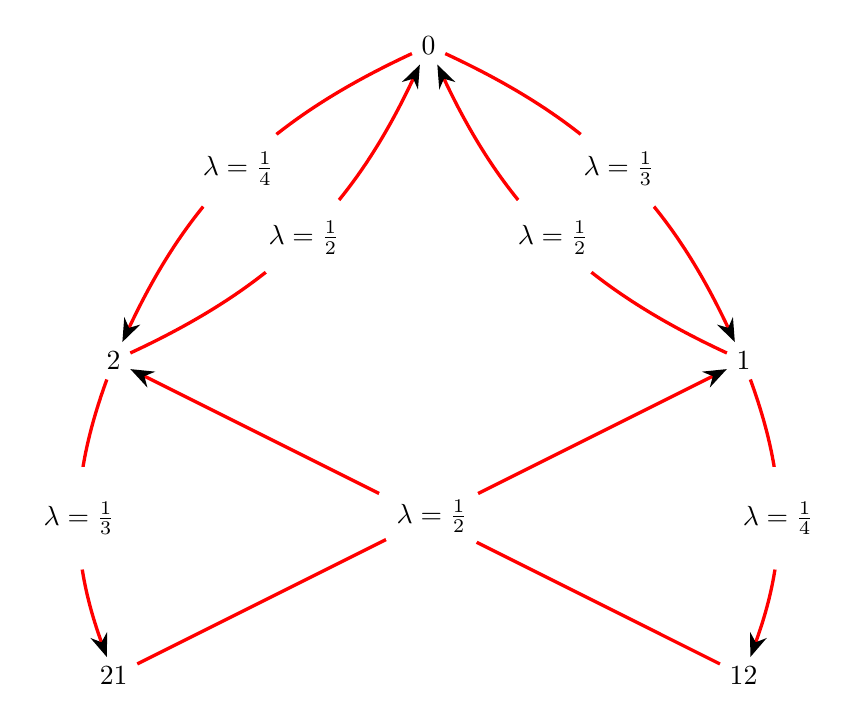
\begin{tikzpicture}
        \node (0) at (0,0) {0};
        \node (1) at (4,-4) {1};
        \node (2) at (-4,-4) {2};
        \node (12) at (4,-8) {12};
        \node (21) at (-4,-8) {21};

        \begin{scope}[>={Stealth[black]},
                every node/.style={fill=white,circle},
                every edge/.style={draw=red,very thick}]
            \path [->] (0)  edge[bend left=20]  node {$\lambda = \frac{1}{3}$} (1);
            \path [->] (0)  edge[bend right=20] node {$\lambda = \frac{1}{4}$} (2);
            \path [->] (1)  edge[bend left=20]  node {$\lambda = \frac{1}{2}$} (0);
            \path [->] (1)  edge[bend left=20]  node {$\lambda = \frac{1}{4}$} (12);
            \path [->] (2)  edge[bend right=20] node {$\lambda = \frac{1}{2}$} (0);
            \path [->] (2)  edge[bend right=20] node {$\lambda = \frac{1}{3}$} (21);
            \path [->] (12) edge                node {$\lambda = \frac{1}{2}$} (2);
            \path [->] (21) edge                node {$\lambda = \frac{1}{2}$} (1);
        \end{scope}
    \end{tikzpicture}
\end{figure}

\subsection{c}
We first observe our model is irreducible and recurrent since all states can be
reached by any other state and vice versa. It's also a finite set of states.

Because of this we can make use of the fact that,
\begin{align*}
    \lim_{t\to\infty} \prob_x(X_t = y) &= \pi_y \\
\end{align*}

Thus we just need to find the limiting distribution at the $y$ state.
In this case we want both $12$ and $21$ then we'll sum these up.

To find the limiting distribution we'll make use of $\pi Q = 0$.
\begin{align*}
    \begin{bmatrix}
        \pi_1 & \pi_2 & \pi_3 & \pi_4 & \pi_5
    \end{bmatrix}
    \begin{pmatrix}
        -7/12        & 1/3          & 1/4          & 0      & 0 \\
        1/2          & -3/4         & 0            & 1/4    & 0 \\
        1/2          & 0            & -5/6         & 0      & 1/3 \\
        0            & 0            & 1/2          & -1/2   & 0 \\
        0            & 1/2          & 0            & 0      & -1/2 \\
    \end{pmatrix}
    &= 0 \\
\end{align*}

We create the following system of equations,
\begin{align}
    -7\pi_1/12 + \pi_2/2 + \pi_3/2 &= 0 \\
    \pi_1/3 - 3\pi_2/4 + \pi_5/2 &= 0 \\
    \pi_1/4 - 5/6\pi_3 + \pi_4/2 &= 0 \\
    \pi_2/4 - \pi_4/2 &= 0 \\
    \pi_3/3 - \pi_5/2 &= 0 \\
\end{align}

Using MATLAB since I don't want to calculate this by hand,
\begin{verbatim}
format rat
A = [-7/12 1/3 1/4 0 0; 1/2 -3/4 0 1/4 0; ...
1/2 0 -5/6 0 1/3; 0 0 1/2 -1/2 0; 0 1/2 0 0 -1/2]
null(A')'
\end{verbatim}

This gives us,
\begin{align*}
    \pi &=
    \begin{bmatrix}
        -437/605 & -287/596 & -649/1797 & -287/1192 & -287/1192
    \end{bmatrix} \\
    &=
    -2384
    \begin{bmatrix}
        1722 & 1148 & 861 & 574 & 574
    \end{bmatrix} \\
    &=
    -\frac{2384}{287}
    \begin{bmatrix}
        6 & 4 & 3 & 2 & 2
    \end{bmatrix} \\
    &=
    -\frac{2384}{4879}
    \begin{bmatrix}
        6/17 & 4/17 & 3/17 & 2/17 & 2/17
    \end{bmatrix} \\
\end{align*}

Thus the probability of both machines being down is $(2+2)/17 = 4/17$.

\subsection{e}
The question asks, knowing we're in state 2, what's the probability we
get to state 0 before state 21.

\begin{align*}
    K_{x,y} &= \frac{q_{x,y}}{q_x} + I\{x=y\} \\
    K_{2,0} &= \frac{q_{2,0}}{q_2} \\
    K_{2,0} &= \frac{1/2}{5/6} \\
    K_{2,0} &= \frac{3}{5} \\
\end{align*}

Likewise we check $K_{2,21}$
\begin{align*}
    K_{2,21} &= \frac{q_{2,21}}{q_2} \\
    K_{2,0} &= \frac{1/3}{5/6} \\
    K_{2,0} &= \frac{2}{5} \\
\end{align*}

Both $K_{2,0}$ and $K_{2,21}$ make up all possibilities for state 2 thus,
the probability that we repair the second machine before the first
machine breaks is $\frac{3}{5}$.

\section{2}
\subsection{a}
There is an unlimited number of customers that could enter the shop thus there
are a countably infinite number of states, we define each state as $i$ where $i$
is the number of customers currently in the store.
This defines the state space of our model.

The initial distribution is to have $\pi^{(0)}_7 = 1$ since we start off with 7 
people.

Since there are countably infinite states we define $\bm{Q}$ as a linear
operator. We redefine our rates in terms of the same units; minutes.
\begin{align*}
    q_{i, i+1} = 1/5 && \forall i \in \mathbb{N} \\
    q_{i, i-1} = 2 && \forall i \in \mathbb{N}\setminus\{0\}
\end{align*}

\subsection{b}
\begin{figure}[H]
    \centering
    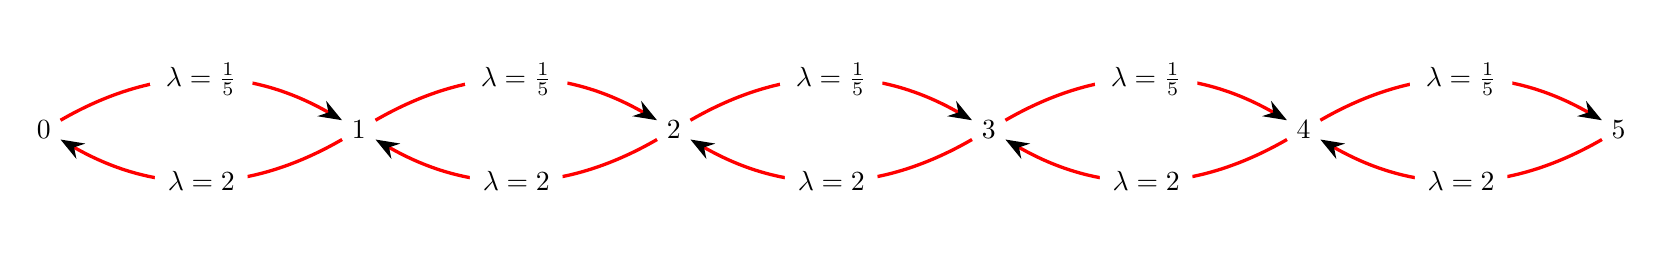
\begin{tikzpicture}
        \node (0) at (0,0)  {0};
        \node (1) at (4,0)  {1};
        \node (2) at (8,0)  {2};
        \node (3) at (12,0) {3};
        \node (4) at (16,0) {4};
        \node (5) at (20,0) {5};

        \begin{scope}[>={Stealth[black]},
                every node/.style={fill=white,circle},
                every edge/.style={draw=red,very thick}]
            \path [->] (0)  edge[bend left=30]  node {$\lambda = \frac{1}{5}$} (1);
            \path [->] (1)  edge[bend left=30]  node {$\lambda = 2$} (0);
            \path [->] (1)  edge[bend left=30]  node {$\lambda = \frac{1}{5}$} (2);
            \path [->] (2)  edge[bend left=30]  node {$\lambda = 2$} (1);
            \path [->] (2)  edge[bend left=30]  node {$\lambda = \frac{1}{5}$} (3);
            \path [->] (3)  edge[bend left=30]  node {$\lambda = 2$} (2);
            \path [->] (3)  edge[bend left=30]  node {$\lambda = \frac{1}{5}$} (4);
            \path [->] (4)  edge[bend left=30]  node {$\lambda = 2$} (3);
            \path [->] (4)  edge[bend left=30]  node {$\lambda = \frac{1}{5}$} (5);
            \path [->] (5)  edge[bend left=30]  node {$\lambda = 2$} (4);
        \end{scope}
    \end{tikzpicture}
\end{figure}


\subsection{c}
Just like in the previous question we can make use of the
\begin{align*}
    \lim_{t\to\infty} \prob_x(X_t = y) &= \pi_y \\
\end{align*}

We'll make use of detailed balance this time since we cannot construct a matrix;
$\pi_x q_{xy} = \pi_y q_{yx}$.
\begin{align*}
    \pi_i q_{i,i+1} &= \pi_{i+1} q_{i+1,i} && \forall i \in \mathbb{N} \\
    \pi_i 1/5 &= \pi_{i+1} 2 \\
    \pi_i &= \pi_{i+1} 10 \\
\end{align*}

Thus if we start from $\pi_0$ we'll have,
\begin{align*}
    \pi_0 &= \pi_1 10 \\
    \pi_1 &= \frac{1}{10} \pi_0 \\
    \pi_2 &= \frac{1}{10^2} \pi_0 \\
    \vdots \\
    \pi_n &= \frac{1}{10^n} \pi_0 \\
\end{align*}

We also recall that $\sum_i \pi_i = 1$. Since our $\pi_i$ create a geometric
series,
\begin{align*}
    \sum_{i=0}^\infty \pi_i &= 1 \\
    \sum_{i=0}^\infty \frac{1}{10^n} \pi_0 &= 1 \\
    \pi_0 \sum_{i=0}^\infty 10^{-n} &= 1 \\
    \pi_0 \frac{1}{1-1/10} &= 1 \\
    \pi_0 \frac{1}{9/10} &= 1 \\
    \pi_0 &= \frac{9}{10} \\
    \pi_1 &= \frac{9}{10^2} \\
    \vdots \\
    \pi_n &= \frac{9}{10^{n+1}} \\
\end{align*}

\subsection{d}
The expected is determined by $\sum_i p \times i$.
\begin{align*}
    &\sum_{i=0}^\infty \frac{9}{10^{i+1}} \times i \\
    &= \sum_{i=0}^\infty \frac{9i}{10^{i+1}} \\
    &= \frac{9}{10} \sum_{i=0}^\infty \frac{i}{10^i} \\
\end{align*}

To evaluate this sum we take a few finite summations,
\begin{align*}
    \sum_{i=0}^3 \frac{i}{10^i} &= 0.123 \\
    \sum_{i=0}^9 \frac{i}{10^i} &= 0.123456789 \\
    \sum_{i=0}^10 \frac{i}{10^i} &= 0.1234567900 \\
    \sum_{i=0}^13 \frac{i}{10^i} &= 0.123456790123 \\
    \vdots \\
    \sum_{i=0}^\infty \frac{i}{10^i} &= \frac{10}{81} \\
\end{align*}

\section{3}
Kolomogorov's axioms are,
probabilities must be non-negative,
$\prob{\Omega} = 1$ and finally the union of events
is equivalent to the sum of each events probability.

We consider a new set $B_i$ where $B_1 = A_1$ but $B_n = A_n \setminus A_{n-1}$.
We note that $B_i$ is in the event set since $A_i^c \cup A_{i-1} \in \mathcal{F}$.
Which means the complement of it is, $A_i \cap A_{i-1}^c = A_i \setminus A_{i-1} \in \mathcal{F}$.

We note that 
\begin{align*}
    \bigcup_{i=1}^n A_i = \bigcup_{i=1}^n B_i
\end{align*}

Since,
\begin{align*}
    \bigcup_{i=1}^n B_i &= \bigcup_{i=1}^n A_{i} \setminus A_{i-1} \\
    &= \bigcup_{i=1}^n A_{i} \cap A_{i-1}^c \\
    &= \bigcup_{i=1}^n A_{i} \\
    &= A_{n}
    && \text{Since they're all subsets of $A_n$} \\
\end{align*}

From here we note each $B_i$ is disjoint and since we have an infinite union
of disjoint sets we have $\prob(\cup_{i=1}^\infty B_i) = \sum_{i=1}^\infty \prob(B_i)$.

\begin{align*}
    \prob(\cup_{i=1}^\infty B_i) &= \sum_{i=1}^\infty \prob(B_i) \\
    \prob(\cup_{i=1}^\infty A_i) &= \sum_{i=1}^\infty \prob(B_i) \\
    \lim_{n\to \infty} \prob(A_n) &= \sum_{i=1}^\infty \prob(B_i)
    && \text{Using the previous two equations we get} \\
    \lim_{n\to \infty} \prob(A_n) &= \prob(\cup_{i=1}^\infty A_i) \\
\end{align*}

\section{5}
$\Omega$ needs to be a set so that's fine.
$\mathscr{B}$ is by definition also an event set since
$\sigma$-algebras are also event sets.

All we require is that
$\mu_X$ is a probability measure.

Kolomogorov's axioms are,
probabilities must be non-negative,
$\prob{\Omega} = 1$ and finally the union of events
is equivalent to the sum of each events probability.

Since our $\mu_X(B)$ is a composition of a predefined probability measure and 
some other function we know such a function holds a domain $\geq 0$.

$X^{-1}$ is the pre-image of the random variable.
Since $\Omega$ in our case is the real number line we have,
$X^{-1}(\mathbb{R}) = \mathbb{R}$.
Following from this we have $\prob$ which is already a probability
measure thus $\prob(\mathbb{R}) = 1$.

Once again, $X^{-1}$ is the pre-image of the random variable.
Thus $X^{-1}(B)$ is asking for all elements in $\Omega (= \mathbb{R})$ that can
map to values in the set $B \subseteq \mathbb{R}$.
We will make use of this fact to prove $X^{-1}(\bigcup A_i) = \bigcup X^{-1}(A_i)$.

Consider $\forall w \in X^{-1}(\bigcup A_i)$ then,
\begin{align*}
    w \in X^{-1}\left(\bigcup A_i\right) &\leftrightarrow w \in X^{-1}\left(\bigcup A_i\right) \\
    &\leftrightarrow X(w) \in \bigcup A_i \\
    &\leftrightarrow X(w) \in A_j \\
    &\text{There must exist one $A_j$ which $w$ is a part of} \\
    &\leftrightarrow w \in X^{-1}(A_j) \\
    &\leftrightarrow w \in \bigcup X^{-1}(A_j) \\
\end{align*}

Thus we have proven that $X^{-1}(\bigcup A_i) = \bigcup X^{-1}(A_i)$. From here
now recall that $\mu_X(B)$ is a composition of a predefined probability measure
and our $X$. Thus $\prob (\bigcup A_i) = \sum \prob(A_i)$ and
$\mu_X (\bigcup A_i) = \sum \mu_X(A_i)$

\end{document}
